	\section{Themengraphen}
\label{sec:topic2graph}
Der nächste Schritt im Ablauf ist die Ermittelung der Themen für die Dokumente und die Erstellung des relationalen Graphen. Insgesamt wurden im Rahmen dieser Diplomarbeit drei Algorithmen entwickelt um aus Themenkookkurrenzen einen Graphen zu erstellen. Diese wurden entwickelt, da bisher keine Algorithmen bekannt sind, die aus Themenkookkurrenzen Graphen erzeugen. Shaffer et. al. \citep{shafferEpistemicFrames} haben einen ähnlichen Algorithmus entwickelt, der Kookkurrenzen von Klassen eines Klassifikationsalgorithmus in einem Graphen kodiert. Die hier entwickelten Algorithmen sind von diesem Algorithmus inspiriert, kodieren jedoch zusätzliche Informationen in den Graphen. So fließen zum Beispiel zusätzlich die Wahrscheinlichkeiten der Themen in die Algorithmen ein.  

Sei $\frame=(\doc_1,\ldots,\doc_f)$ ein Frame des Korpus. Dann wird anhand des gelernten Themenmodells für jedes Dokument inferiert, welche Themen in diesem vorkommen. Dies geschieht anhand der Inferenz für ungesehene Dokumente in Abschnitt \ref{subsec:infUnseen} des Grundlagenkapitels. So erhält man für jedes Dokument $\doc_i$ in Frame $\frame$ eine Themenverteilung $\docTopicDist{i}$. Anhand der Themenverteilung der Dokumente in den Frames kann ein Graph aufgebaut werden, der die Kookkurrenz und die Wahrscheinlichkeit der Themen in einem Frame kodiert. Die Knoten des Graphen stellen dabei die Themen dar und die Kanten kodieren die Kookkurrenz der Themen in einem Frame. 

\subsection{Vollständiger Graph (\CST)}
\label{subsec:cst}
Der erste Algorithmus erstellt einen vollständig verbundenen Graphen, dessen Kanten mit der inversen Häufigkeit des Themenauftretens gewichtet sind. Die Themen, deren Wahrscheinlichkeiten größer als ein Schwellwert $\epsilon$ sind, werden als Knotenmenge aufgefasst und es wird für jedes Themenpaar gezählt, wie oft es zusammen auftritt. In dem Pseudocode Algorithmus \ref{lst:countingSimpleTopicToGraph} wird der Algorithmus dargestellt. 

Es wird über alle Dokumente $\doc_m \in \frame$ iteriert und die Themen $\docTopic_k$, deren Wahrscheinlichkeit $\docTopicProb{m}{k}$ im Dokument größer als der gewünschte Schwellwert ist, werden als Knoten in den Graphen eingefügt. Dann werden für alle diese Themen $\docTopic_k$ Kanten zu allen anderen Knoten $v$ gezogen. Wenn die Kante im Graphen schon vorhanden ist, muss ihr Gewicht angepasst werden. Für jede bereits vorhandene Kante wird das Gewicht von $\frac{1}{n}$ auf $\frac{1}{n+1}$ angepasst. Dazu wird in Zeile 6 erst einmal das aktuelle Gewicht der Kante ausgelesen. Anhand des alten Gewichtes kann man feststellen, wie oft die Kante schon in den Graphen eingefügt wurde. Daraus berechnet sich dann das neue Gewicht. Der Vorteil besteht darin, dass man sich eine Datenstruktur erspart, die zählt, wie oft eine Kante bereits eingefügt wurde und, dass eine Iteration über alle Kanten wegfällt. Wenn die Kante im Graphen noch nicht vorhanden ist, wird sie hinzugefügt und bekommt ein initiales Gewicht von eins.

\begin{algorithm}[ht]
\begin{algorithmic}[1]
\STATE $V = \emptyset, E = \emptyset$
\FORALL{$\doc_m \in \frame$}
  \STATE $V = V \cup \left\lbrace k | \docTopicProb{m}{k} > \epsilon \right\rbrace$
  \FOR{$k \in \left\lbrace \docTopicProb{m}{k} > \epsilon \right\rbrace$}
    \FOR{$v \in V$}
      \IF{$\left\lbrace v,k \right\rbrace \in E \wedge v \neq k$}
        \STATE $oldWeight = \edgeWeight{\left\lbrace v,k \right\rbrace}$ 
        \STATE $count = \frac{1}{oldWeight}$	
	    \STATE $\edgeWeight{\left\lbrace v,k \right\rbrace} = \frac{1}{count + 1}$
      \ELSE
        \STATE $E = E \cup \left\lbrace \left\lbrace v,k \right\rbrace \right\rbrace$
        \STATE $\edgeWeight{\left\lbrace v,k \right\rbrace} = 1$
      \ENDIF
    \ENDFOR
  \ENDFOR
\ENDFOR 
\end{algorithmic}
\label{lst:countingSimpleTopicToGraph}
\caption{Vollständig verbundener Graph (\CST)}
\end{algorithm}

Alternativ kann der Graph in mathematischer Mengenschreibweise angegeben werden, wenn man festhält, wie oft ein Thema als Knoten eingefügt wurde. Dazu sei $G=(V,E)$ ein Graph mit $V$ als Knotenmenge und $E$ als Kantenmenge. Die Knotenmenge $V$ ist hier ein Multiset, das festhält, wie oft ein Element in die Menge eingefügt wurde. Die Anzahl der einzelnen Mengenelemente $x$ wird durch die Funktion $count(x)$ angegeben. 

Die Knoten des Graphen ergeben sich aus den Themen, für die die Dokumentwahrscheinlichkeit größer als ein Schwellwert $\epsilon$ ist.
\begin{equation}
V = \bigcup_{\doc_m \in \frame} \left\{ k | \docTopicProb{m}{k} > \epsilon\right\}
%\label{eq:countingSimpleTopicToGraphNodes}
\end{equation}

Zwischen allen Knoten im Graphen werden dann Kanten gezogen. Dabei sind Zyklen im Graphen nicht erlaubt. Es ist:
\begin{equation}
E = \left\{ \{i,j\} | i,j \in V, i \neq j \right\}
\end{equation}

Das Kantengewicht wird als die inverse Anzahl der Kookkurrenz von Themen definiert. Die Anzahl der Kookkurrenzen ist dabei das Minimum der Auftreten der Knoten einer Kante. 
\begin{equation}
\omega(\{i,j\}) = \frac{1}{\min \{count(i),count(j)\} } 
\end{equation}

In Abbildung \ref{fig:simpleFrameToGraph} ist der resultierende Graph eines Frames mit vier Dokumenten abgebildet. Die Zahlen in den Knoten geben den Index des Themas und die Zahlen in Klammern die Anzahl des Auftretens des Themas an. 

\begin{figure}
\centering
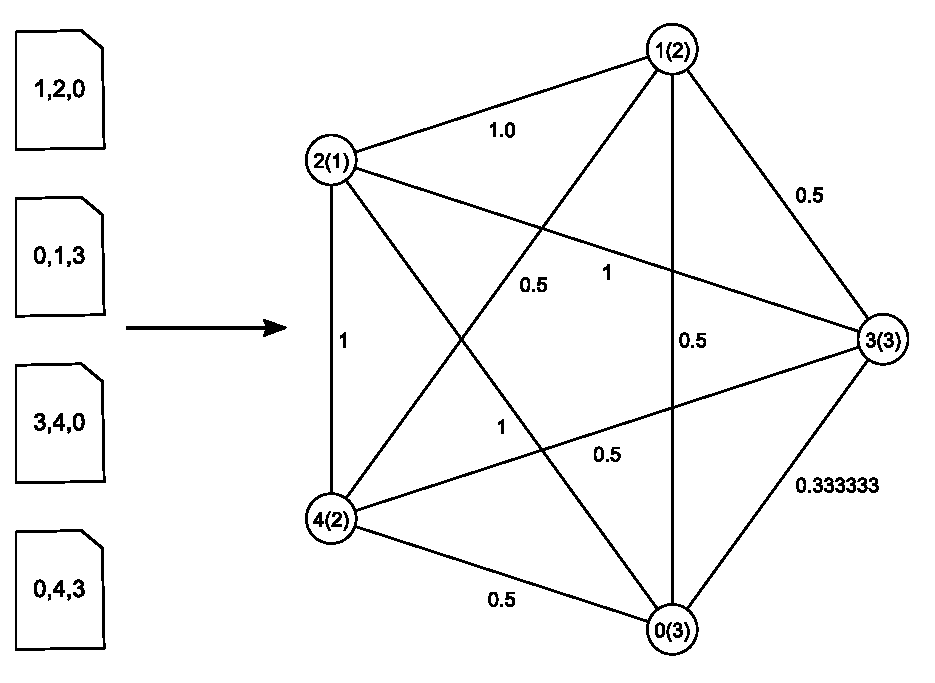
\includegraphics[scale=.6]{images/content/05_workflowTime/simpleFrameToGraph}
\caption{Erzeugung eines Graphen aus Dokumenten und den zugewiesenen Themen mittels des Algorithmus \CST}
\label{fig:simpleFrameToGraph}
\end{figure}

\subsection{Dokumentzentrierter Graph (\CDC)}
\label{subsec:cdc}

Der zweite Algorithmus erzeugt keinen vollständig verbundenen Graphen. 
Im Einzelnen werden, ähnlich wie im vorhergehenden Algorithmus \CST, die Themen der Dokumente mit einer Wahrscheinlichkeit größer als ein angegebener Schwellwert als Knoten in den Graphen eingefügt. Allerdings werden nur noch Kanten gezogen, wenn die Themen in den Dokumenten vorkommen. Da gleiche Themen oft in verschiedenen Dokumenten vorkommen, ergibt sich wieder ein zumindest schwach zusammenhängender Graph. Ein Thema, das in allen Dokumenten vorkommt, wird mit allen anderen Themen verbunden sein. Dies kann man in Abbildung \ref{fig:documentCentricFrameToGraph} sehen. Hier kommt Thema 1 in jedem Dokument vor und verbindet deshalb alle Dokumentsubgraphen miteinander. Thema 6 und 4 kommen in zwei Dokumenten vor und verbinden somit zwei Dokumente. Hier ist es jedoch möglich, dass ein Dokument nur aus Themen zusammengesetzt ist, die in keinem anderen Dokument vorkommen. So entsteht ein nicht verbundener Graph. 

\begin{figure}[ht]
\centering
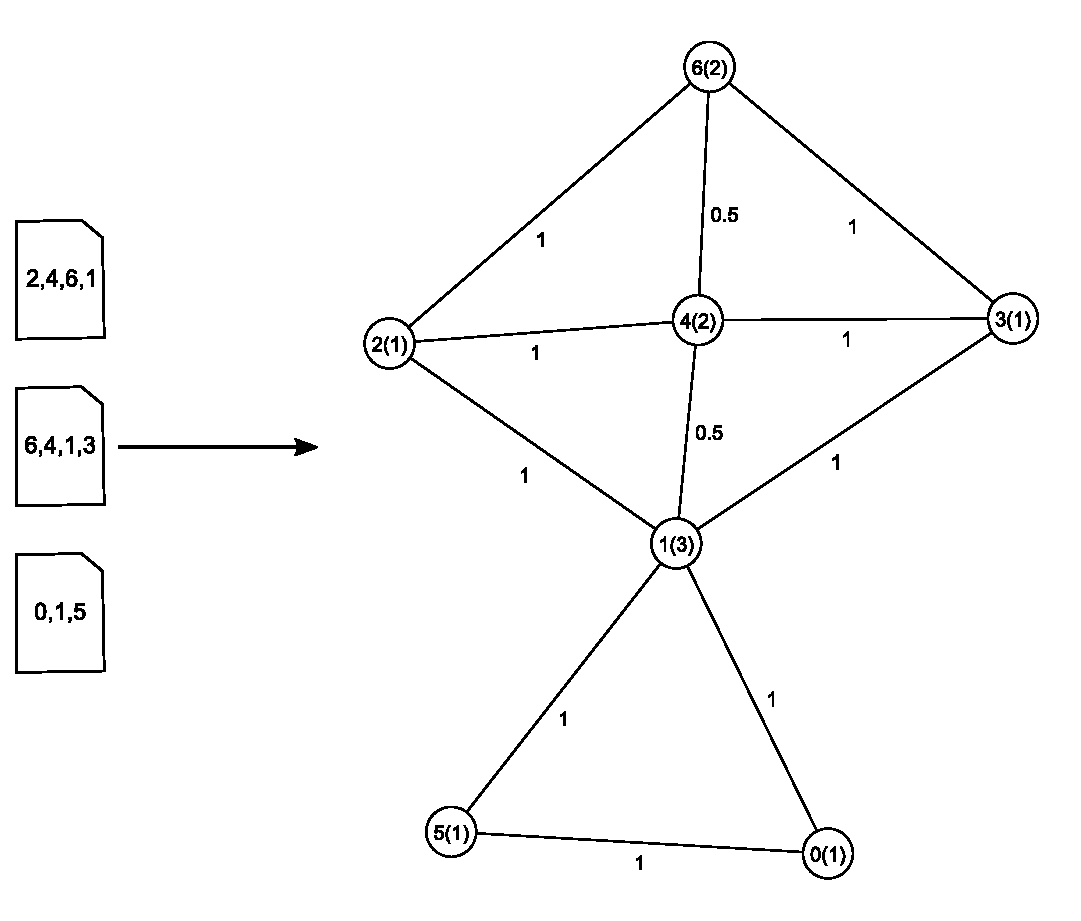
\includegraphics[scale=.6]{images/content/05_workflowTime/documentCentricFrameToGraph.eps} 
\caption{Erzeugung eines Graphen aus Dokumenten und den zugewiesenen Themen mittels des Algorithmus \CDC}
\label{fig:documentCentricFrameToGraph}
\end{figure}

Der Algorithmus zur Erstellung der Graphen funktioniert ähnlich zum vorhergehenden. Es wird für jedes Dokument ein vollständig verbundener Subgraph erstellt. Dies wird in Algorithmus \ref{lst:documentCentricFrameGraph}, in den Zeilen 3 bis 16 codiert. Dort werden auch die Themen $\docTopic_k$ als Knoten eingefügt, deren Wahrscheinlichkeit $\docTopicProb{m}{k}$ größer als der Schwellwert ist. Dann wird für jeden Knoten im Subgraphen $G_m=(V_m,E_m)$ eine Kante zu jedem anderen Knoten gezogen. Wenn eine Kante im globalen Graphen $G=(V,E)$ schon vorhanden ist, muss das Gewicht dieser Kante angepasst werden. Dazu wird analog wie in Algorithmus \ref{lst:countingSimpleTopicToGraph} erst die Anzahl der Vorkommen dieser Kante bestimmt und dann das Gewicht angepasst (siehe Zeile 8-10). Wenn der Subgraph $G_m$ erstellt wurde, werden die Knotenmengen und Kantenmengen des Subgraphen mit dem globalen Graphen vereinigt. 

\begin{algorithm}[ht]
\begin{algorithmic}[1]
\STATE $V = \emptyset, E = \emptyset$
\FORALL{$\doc_m \in \frame$}
  \STATE $V_m = \emptyset, E_m = \emptyset$
  \STATE $V_m = \left\lbrace k | \docTopicProb{m}{k} > \epsilon \right\rbrace$
  \FOR{$k \in V_m$}
    \FOR{$v \in V_m$}
      \IF{$\left\lbrace v,k \right\rbrace \in E \wedge v \neq k$}
        \STATE $oldWeight = \edgeWeight{\left\lbrace v,k \right\rbrace}$ 
        \STATE $count = \frac{1}{oldWeight}$	
	    \STATE $\edgeWeight{\left\lbrace v,k \right\rbrace} = \frac{1}{count + 1}$
      \ELSE
        \STATE $E_m = E_m \cup \left\lbrace \left\lbrace v,k \right\rbrace \right\rbrace$
        \STATE $\edgeWeight{\left\lbrace v,k \right\rbrace} = 1$
      \ENDIF
    \ENDFOR
  \ENDFOR
  \STATE $V = V \cup V_m$
  \STATE $E = E \cup E_m$
\ENDFOR 
\end{algorithmic}
\label{lst:documentCentricFrameGraph}
\caption{Dokument zentrischer Graphenalgorithmus (\CDC)}
\end{algorithm}

Hier ist es gleichfalls möglich, den Algorithmus direkt in Mengenschreibweise anzugeben. Es muss wieder festgehalten werden, wie oft ein Thema in die Knotenmenge eingefügt wurde. Die Knotenmenge ist die gleiche wie im vorhergehenden Algorithmus: Sie enthält alle Themen, deren Dokument-Wahrscheinlichkeit größer als $\epsilon$ ist. 
\[
V = \bigcup_{\doc_m \in \frame} \left\{ k | \docTopicProb{m}{k} > \epsilon\right\}
\]

Allerdings wird nicht mehr jeder Knoten mit allen anderen Knoten verbunden. Es werden nur noch die Knoten verbunden, für die gilt, dass sie im selben Dokument vorkommen und ihre Dokumentwahrscheinlichkeit größer als der geforderte Schwellwert ist. 
\[
E = \bigcup_{\doc_m \in \frame} \left\{ {i,j} | \docTopicProb{m}{i} > \epsilon \wedge \docTopicProb{m}{j} > \epsilon, i \neq j \right\}
\]

Die Kantengewichte wiederum werden analog zum vorhergehenden Algorithmus bestimmt. 
 \[
 \omega(\{i,j\}) = \frac{1}{min \{count(i),count(j)\} } 
 \]


\subsection{Graph mit Themenwahrscheinlichkeit (\TPR)}
\label{subsec:tpr}

Der nächste Algorithmus berücksichtigt die Wahrscheinlichkeit der Themen in den Dokumenten. Anhand der Wahrscheinlichkeiten werden die Gewichte der Kanten berechnet. Ansonsten wird der Graph wie in Abschnitt \ref{subsec:cdc} aufgebaut. Zuerst werden alle Themen des aktuellen Dokuments, deren Wahrscheinlichkeit größer als $\epsilon$ sind, als Knoten in den Subgraphen eingefügt. Danach werden zwischen allen Knoten des Subgraphen Kanten gezogen. Wenn die Kante im globalen Graphen noch nicht existiert, wird sie im Subgraphen hinzugefügt mit einem initialen Gewicht das dem inversen F-Wert der beiden Themenwahrscheinlichkeiten $k$ und $v$ im Dokument $m$ entspricht. Ist die Kante im globalen Graphen schon vorhanden, wird das Gewicht folgendermaßen angepasst: Das neue Gewicht berechnet sich als Produkt des alten Gewichtes mit dem inversen F-Wert der Themenwahrscheinlichkeiten der beiden Themen $k$ und $v$ im Dokument $m$.
\begin{equation}
1 - \frac{2 \cdot \docTopicProb{m}{v} \cdot \docTopicProb{m}{k}}{\docTopicProb{m}{v} + \docTopicProb{m}{k}}
\label{eq:topicProbWeightFScore}
\end{equation}
Der inverse F-Wert in Gleichung \ref{eq:topicProbWeightFScore} nähert sich für zwei hohe Wahrscheinlichkeiten $\docTopicProb{m}{v}$ und $\docTopicProb{m}{k}$ Null an und für zwei niedrige Wahrscheinlichkeiten Eins an. Das heißt, zwei Knoten mit hoher Wahrscheinlichkeit liegen näher beieinander als zwei Knoten mit niedriger Wahrscheinlichkeit. Durch die Anpassung der Gewichte wird die Distanz zweier Themenknoten, die häufiger zusammen auftreten, kleiner. Dies ist für die später berechneten Zentralitätsindizes wichtig.

\begin{algorithm}[ht]
\begin{algorithmic}[1]
\STATE $V = \emptyset, E = \emptyset$
\FORALL{$\doc_m \in \frame$}
  \STATE $V_m = \emptyset, E_m = \emptyset$
  \STATE $V_m = \left\lbrace k | \docTopicProb{m}{k} > \epsilon \right\rbrace$
  \FOR{$k \in V_m$}
    \FOR{$v \in V_m$}
      \IF{$\left\lbrace v,k \right\rbrace \in E \wedge v \neq k$}
        \STATE $\edgeWeight{\left\lbrace v,k \right\rbrace} = \edgeWeight{\left\lbrace v,k \right\rbrace} \cdot \left( 1 - \frac{2 \cdot \docTopicProb{m}{v} \cdot \docTopicProb{m}{k}}{\docTopicProb{m}{v} + \docTopicProb{m}{k}}\right)$
      \ELSE
        \STATE $E_m = E_m \cup \left\lbrace \left\lbrace v,k \right\rbrace \right\rbrace$
        \STATE $\edgeWeight{\left\lbrace v,k \right\rbrace} = 1 - \frac{2 \cdot \docTopicProb{m}{v} \cdot \docTopicProb{m}{k}}{\docTopicProb{m}{v} + \docTopicProb{m}{k}}$
      \ENDIF
    \ENDFOR
  \ENDFOR
  \STATE $V = V \cup V_m$
  \STATE $E = E \cup E_m$
\ENDFOR 
\end{algorithmic}
\label{lst:topicProbFrameGraph}
\caption{Graph mit Themenwahrscheinlichkeit (\TPR)}
\end{algorithm}

Die Definition des Graphen in Mengenschreibweise ist wie folgt. Die Knoten des Graphen sind wieder diejenigen Themen deren Wahrscheinlichkeit in einem Dokument des Frames größer als $\epsilon$ ist.
\[
V = \bigcup_{\doc \in \frame} \left\{ k | \docTopicProb{m}{k} > \epsilon\right\}
\]

Die Kanten werden zwischen Themenknoten gezogen, die in demselben Dokument vorkommen, analog zum vorhergehenden Algorithmus.
\[
E = \bigcup_{\doc_m \in \frame} \left\{ {i,j} | \docTopicProb{m}{i} > \epsilon \wedge \docTopicProb{m}{i} > \epsilon, i \neq j \right\}
\]

Das Gewicht einer Kante von $i$ nach $j$ berechnet sich als das Produkt des inversen F-Wertes der Wahrscheinlichkeit des Themas $i$ und $j$ in allen Dokumenten, in denen die Themen $i$ und $j$ zusammen auftreten. Dies entspricht dem mehrmaligen Einfügen einer Kante, wie es im Algorithmus aufgeführt wird.
\[
\omega(\{i,j\}) = \prod_{m : \docTopicProb{m}{i} > \epsilon \wedge \docTopicProb{m}{j} > \epsilon} 1 -
\frac{2 \cdot \docTopicProb{m}{i} \cdot \docTopicProb{m}{j}}{\docTopicProb{m}{i} + \docTopicProb{m}{j}}
\]

